\documentclass[tikz, margin=3mm]{standalone}
\usepackage{chemformula}

%######################%
% Lighter Blue palette %
%######################%

%----------------------------------------------------------------------------------
\definecolor{lightstrongblue}{HTML}{4E7EC5}
\definecolor{lightnormalblue}{HTML}{79A0DA}
\definecolor{lightfadingblue}{HTML}{98B4E3}
\definecolor{lightweakblue}{HTML}{B9CBEC}
\definecolor{almostwhiteblue}{HTML}{CAD7F0}
%----------------------------------------------------------------------------------


%##############################%
% Darker blue palette elements %
%##############################%

%----------------------------------------------------------------------------------
\definecolor{darkstrongblue}{HTML}{214598} 
\definecolor{neutralblue}{HTML}{4564B7}
\definecolor{fadedblue}{HTML}{6E7FC7}
\definecolor{whitishblue}{HTML}{9AA2D8}
\definecolor{paleblue}{HTML}{CACCEB}
%----------------------------------------------------------------------------------

\usetikzlibrary{arrows.meta,
                chains,
                positioning,
                shapes.geometric
                }
                
\tikzstyle{startstop} = [rectangle, rounded corners, 
minimum width=3cm, 
minimum height=1.5cm,
draw=black,
text width=35mm,
align=center,
font=\linespread{1.4}\selectfont,
fill=darkstrongblue!30]

\tikzstyle{inpout} = [trapezium, 
trapezium stretches=true,
trapezium left angle=70, 
trapezium right angle=110, 
minimum width=3cm, 
minimum height=1.5cm,
draw=black,
text width=35mm,
align=center,
font=\linespread{1.4}\selectfont,
fill=neutralblue!30]

\tikzstyle{proc} = [rectangle, 
minimum width=3cm, 
minimum height=1.5cm,
draw=black,
align=center,
text width=35mm,
font=\linespread{1.4}\selectfont,
fill=fadedblue!30]

\tikzstyle{dec} = [diamond, 
minimum width=3cm, 
minimum height=1.5cm, 
text centered, 
draw=black,
text width=35mm,
align=center,
font=\linespread{1.4}\selectfont,
fill=whitishblue!30]

\tikzstyle{arrow} = [thick,->,>=stealth]

\begin{document}
\begin{tikzpicture}

\node (start) [startstop] {\Large{$\ch{AnAd2}$\\ 4-picoline\\ Acetic anhydride}};
\node (proc1) [proc, right of=start, xshift=4.5cm] {\Large{${100^\circ C}$\\ Reflux}};
\node (proc2) [proc, right of=proc1, xshift=4.5cm] {\Large{A.T \\ Stirring}};
\node (proc3) [proc, right of=proc2, xshift=4.5cm] {\Large{Filtration}};
\node (proc4) [proc, right of=proc3, xshift=4.5cm] {\Large{Recristalization \\ DMF}};
\node (stop) [startstop, right of=proc4, xshift=4.5cm] {\Large{Centrifugation\\ An2Py}};
    
\draw [arrow] (start) -- (proc1);
\draw [arrow] (proc1) -- node[anchor=north] {\Large{12h}} (proc2);
\draw [arrow] (proc2) -- node[anchor=north] {\Large{12h}} (proc3);
\draw [arrow] (proc3) -- (proc4);
\draw [arrow] (proc4) -- (stop);

%\draw [arrow] (d) -- node[anchor=east] {yes} (e);
    
\end{tikzpicture}
\end{document}
